\usetikzlibrary{arrows}
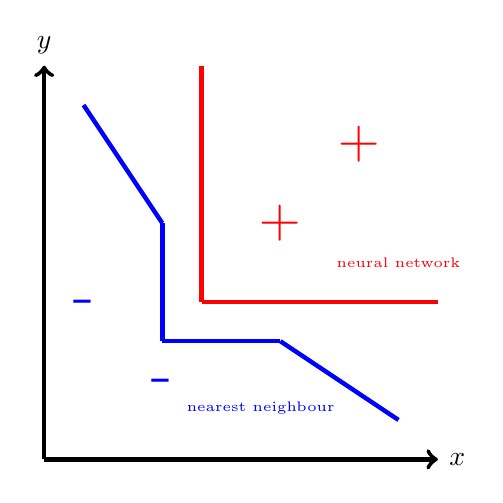
\begin{tikzpicture}


\draw[->,ultra thick] (0,0)--(5,0) node[right]{$x$};
\draw[->,ultra thick] (0,0)--(0,5) node[above]{$y$};

\node [text=blue] at (1.5,1) {\Huge -};
\node [text=blue] at (0.5,2) {\Huge -};
\node [text=red] at (3,3) {\huge +};
\node [text=red] at (4,4) {\huge +};

\draw[red,ultra thick] (2,5)--(2,2);
\draw[red,ultra thick] (5,2)--(2,2);


\draw[blue,ultra thick] (0.5,4.5)--(1.5,3);
\draw[blue,ultra thick] (1.5,3)--(1.5,1.5);
\draw[blue,ultra thick] (1.5,1.5)--(3,1.5);
\draw[blue,ultra thick] (3,1.5)--(4.5,0.5);

\node[red] at (4.5,2.5) {\tiny neural network};
\node[blue] at (2.75,0.65) {\tiny nearest neighbour};

\end{tikzpicture}+